\lab{Python}{Object Oriented Programming}{Object Oriented Programming}
\label{lab:OOP}
\objective{Teach how to use OOP in Python and illustrate the uses of OOP in programming graphical user interfaces}

\section*{Programming Paradigms}

Writing readable code is one of the best skills a programmer can learn.
Good code should not only perform well, but should be understnadable to others.
Organization is key to clarity, and common ways of organizing code are called \emph{programming paradigms}.
\emph{Object oriented programming} (OOP) is one of these paradigms.
It allows us to model and replicate organization and structure from real life.
OOP also allows us to create a ``black box'' that can be used without understanding the inner workings.

Because of these advantages, obeject oriented programming has become a prominent and important programming paradigm used to simplify, organize, and clarify code. 
In this lab we will first learn how to use OOP with Python and implement some simple examples. 
Then we will learn about \emph{graphical user interfaces} (GUI) and OOP's uses in implementing them.


\begin{comment}
A way of organizing a program is often called a ``paradigm."

Paradigms are designed to create better code by structuring or organizing the code in a more meaningful way.
Code without any structure is often referred to as ``spaghetti code.''
Spaghetti can be very easy to write, but very difficult to understand or modify.
\emph{Structured programming} emphasizes the use of programming structures to select or repeat the execution of blocks of code.
It is good practice to structure your programs in such a way that they are easy to understand, extend, or reuse.
Making extensive use of procedures (or subfunctions) is a characteristic of \emph{procedural programming}.
The work of the program is done in the subfunctions with one main function supervising the calling of each subfunction.

Another important, albeit specialized, paradigm is \li{object oriented programming} (or OOP).
The concept of object oriented programming is to model a problem as the interaction of a collection of objects.
There are many other paradigms such as declarative, event-driven, and array programming.
\end{comment}



\section*{Fundamental Concepts}

\begin{comment}
At its core, object oriented programming relies on the manipulation and coordination of objects.
An object represents a piece of code that tracks a state and provides methods for discovering or altering the state.


There are a few concepts that define object oriented programming

\begin{itemize}

\item Abstraction - appropriate representation of states and data

\item Encapsulation - independent behavior

\item Inheritance - relations between objects

\end{itemize}

The general advantage of using these concepts is that it helps with organizing code.
``Abstraction" permits the presentation of only necessary details about an object to the user.
For example, when we ask someone if they own a computer, we can use abstraction to ask the question ``Do you own a computer?'' rather than asking about each and every combination of hardware that we could classify as a computer.
Inheritance helps us easily achieve this abstraction.
We could have an object called \li{Computer}.
Various brands would then subclass, or inherit, the properties of \li{Computer}.
We could continue by having each product line inherit from their respective brands, until we arrive at the product level.
Then each individual product would represent an instantiation of that product's class.
%Need graphic
Encapsulation means each function contains all of the data it needs to calculate a result.
Encapsulation is used to avoid the use of global data structures and makes managing data involved in computation more convenient.
\end{comment}

At its core, object oriented programming relies on the manipulation and coordination of objects.
Objects are abstractions of real life ``actors'' that can perfom work, report on and change thier state, and communcate with other objects in the system. %Change direct quote from wikepedia
\emph{Abstraction} is one of the major concepts in OOP.
Python, like most modern programming languages, supports object oriented programming concepts.
However, unlike other programming languages everything in Python is an object.

An object contains variables and provides methods for discovering or altering those variables.
This is grouping is called \emph{encapsulation}, another important concept in OOP.
Strings, lists, and even integers are examples of objects in Python, which is why they have \emph{methods}, functions that belong specifically to those objects.
We can create our own objects in Python by defining a \emph{class}.
A class is a blueprint that describes how to create an object.

\begin{lstlisting}
class Backpack(object):
    pass
\end{lstlisting}

We now have a class \li{Backpack} which contains nothing.
We put \li{object} in parenthesis to make our \li{Backpack} a subclass of Python's \li{object} class.
This is an example of \emph{inheritance}, the third important concept in OOP.
Because our backpack class is a subclass of Python's \li{object} class, it inherits properties and methods implemented in the \li{object} class.

We can create \li{Backpack} objects by running something like \li{b = Backpack()}, but we can't really do anything with them.
The variable \li{b} would then be an \emph{instance} of type \li{Backpack}.
Let's define an initial state for our object.

\begin{lstlisting}
class Backpack(object):
    def __init__(self):
        self.color = 'black'
\end{lstlisting}

Let's explain what's going on here.
First, we defined a method.
It can be called on instances of our class but on nothing else.
The \li{__init__} method is defined for all objects and is executed immediately after the object is created.
Its purpose is to set the initial state of the object.
The \li{self} is a reference to the current instance of the class.
All class methods take \li{self} as their first argument.
In our \li{__init__} methods, we are telling it to set the backpack's color to black.
Instead, let's allow the user to choose a different color, but we will still make black the default.

\begin{lstlisting}
class Backpack(object):

    # __init__ will take color as an argument
    # color = 'black' means that if nothing is given, the color is automatically set to black.
    def __init__(self, color='black'): 
        self.color = color
\end{lstlisting}

The variable \li{self.color} is an instance variable. It is defined for a particular instance of a backpack.
We can also change it outside of the class definition.
Let's instantiate a \li{Backpack} object of the color purple.
If we do not specify than it will default to black.

\begin{lstlisting}
b = Backpack(color='purple')
a = Backpack()
print b.color #prints 'purple'
print a.color #prints 'black'
a.color = 'yellow'
print a.color #prints 'yellow'
\end{lstlisting}


Finally, lets add some methods and additional state variables.

\begin{lstlisting}
class Backpack(object):
    def __init__(self, color='black'):
        self.color = color
        # This creates an empty list when a backpack is created. 
        # It will store the backpack's contents.
        self.contents = []

    def put(self, item):
        # This adds ``item'' into our contents list. 
        # self.contents accesses the instance variable.
        # Then .append() uses list's append function to add ``item'' to the end of the list.
        self.contents.append(item) 
        
        
    def take(self, item):
        # The index() method returns the index of ``item''
        # Then the pop() method removes the item at the given index.
        return self.contents.pop(self.contents.index(item)) 
        
        
\end{lstlisting}

Now that we have defined methods for our \li{Backpack} class, we can interact with it.


\begin{lstlisting}
b = Backpack(color='green')
print b.color #prints `green'
print b.contents # prints `[]'
b.put(5)
b.put(3)
b.put(9)
b.put(1)
print b.contents #prints `[5, 3, 9, 1]'
b.take(3)
print b.contents #prints `[5, 9, 1]'
\end{lstlisting}

Our \li{Backpack} class is an example of \emph{encapsulation}.
Encapsulation refers to bundling data and the methods that are used on that data.
In \li{Backpack}, our data is the color and list of contents while the methods are \li{put()} and \li{take()}.

\begin{problem}
Create a class called \li{People} that allows us to keep track of professors and students.
Each instance of \li{People} should have a variable that can be set to `Student' or `Professor' and a list to keep track of thier classes.
Include methods that allow us to add and take away a classes.
\label{School}
\end{problem}

One ability that our classes are missing is the ability to interact with common operations and functions.
Python's objects such as strings, lists, integers can interact with \li{print},  $ =, - , >, \text{and} <$.
Right now, if we used \li{print} on an instance of \li{Backpack}, Python would not know how to interpret it as a string.
Similarly, Python would not know how to compare one backpack to another using $ =, - , >, \text{and} <$.
We can fix this by using \emph{magic methods}.
Magic methods are special methods that add fucntionality to classes.
Magic methods can be recognized by the double underscores in their names.

Let's add two magic methods to \li{Backpack}. 
The \li{__repr__} method tells Python how to represent our class as a string. 
Then we will be able to call \li{print b} and it will print our backpack, b.
The \li{__lt__} methods will implement the $<$ operator, letting us compare two backpacks.

\begin{lstlisting}
class Backpack(object):
    def __init__(self, color='black'):
    	self.color = color
    	self.contents = []
        
    def put(self, item):
    	self.contents.append(item)
        
    def take(self, item):
    	return self.contents.pop(self.contents.index(item)) 

    def __repr__(self):
    '''Tells the class how to represent the Backpack object as a string'''
    	#Returns a string version of the contents list
    	 return str(self.contents)
             
   
   def __lt__(self, other):
   '''Compares the length of the two backpack's contents lists.'''
     	 return len(self.contents) < len(other.contents)

\end{lstlisting}

The other comparison operators are implemented in a similar way.
Now let's test our magic methods.

\begin{lstlisting}
b = Backpack(color='green')
c = Backpack(color='yellow')
b.put(2)
b.put(5)
c.put(7)
c.put(1)
c.put(8)
print b # prints `[2,5]'
print c # prints `[7,1,8]'
# Should return True, sending us into the if branch.
if b < c: 
	print 'b is less than c'

\end{lstlisting}

For more information on creating methods and magic methods read the official Python docs, at \url {http://docs.python.org/2/reference/datamodel.html} or another helpful reference at \url{http://www.rafekettler.com/magicmethods.html}.
This information may be helpful in solving Problem \ref{prob:complexNum}.

\begin{problem}
Create a \li{ComplexNumber} object that supports the basic operations of a complex number.
You must implement methods that will compare, add, subtract, multiply, divide, and conjugate complex numbers.
Also, implement a \li{norm()} method that will calculate the euclidean distance between two points on the complex plane.
\label{prob:complexNum}
\end{problem}

\section*{Graphical User Interfaces}

GUI's are a powerful tool for creating applications that users can interface with.
PySide is a helpful library to build GUI's.
From PySide, we will used two modules, QtGui and QtCore.
QtCore has functions that will help us implement the inner workings of our GUI while QtGui will allows us to implement the graphics and interface. 
To walk through the main ideas behind building a GUI, we will create a simple program that will display inputted text.

\begin{lstlisting}
from PySide import QtGui, QtCore

class Printer(QtGui.QWidget): 
	#This class inherits from the QWidget class found in the QtGui module.
	def __init__(self):
		# Calls the __init__ method from QWidget, the super class of BackpackInterface.
		super(Printer, self).__init__() 

\end{lstlisting}

\emph{Widgets} are what allows the magic to happen in GUIs.
Widgets in Qt are objects that represent various elements of a GUI.
They keep track of drawing and refreshing the graphical display of the elements as well as abstracting the behavior and defining ways to act with other widgets.
For example, when you push a button or enter text, it is the widgets that realize it and cause changes.
In our \li{Printer} we will use \li{QLineEdit} and \li{QLabel}.

\begin{lstlisting}
from PySide import QtGui, QtCore

class Printer(QtGui.QWidget):
	def __init__(self):
		super(Printer, self).__init__() 
		#calls the _initUI function
		self._initUI()
	
	def _initUI(self): 
		'''Creates the widgets and tells them how to interact'''
		
		# creates a class variable called textBar that is a QLineEdit widget 
		self.textBar = QTGui.QLineEdit()
		# creates a class variable called label that is a QLabel widget
		self.label = Qt.Gui.QLabel()

\end{lstlisting}

Now that we have our widgets, we need to tell them how to communicate.
Qt uses a system of \emph{signals} and \emph{slots}.
When a button is pushed or text is entered, a widget throws a signal.
We can specify what slot catches the signal.
In our case, we want a function to catch the signal, update the displayed text, and clear the text bar.

\begin{lstlisting}
from PySide import QtGui, QtCore

class Printer(QtGui.QWidget):
	def __init__(self):
		super(Printer, self).__init__() 
		self._initUI()

	def _initUI(self): 
		self.textBar = QTGui.QLineEdit()
		self.label = Qt.Gui.QLabel()
		
		# When return is pressed in the textBar, it sends a signal and we go into the function updateText.
		self.textBar.returnPressed.connect(self.updateText)
	
		
	def updateText(self):
	'''Updates what text is displayed and clears the textBar'''
		self.label.setText(self.textBar.displayText())
		self.textBar.clear()

\end{lstlisting}

Next we need to set the layout and create a function that can be called from the command line.

\begin{lstlisting}
from PySide import QtGui, QtCore
import sys

class Printer(QtGui.QWidget):
	def __init__(self):
		super(Printer, self).__init__() 
		self._initUI()

	def _initUI(self): 
		self.textBar = QTGui.QLineEdit()
		self.label = Qt.Gui.QLabel()
		
		self.textBar.returnPressed.connect(self.updateText)
	
		# Creates a vertical box layout
		# It will stack all widgets added to it vertically
		vbox = QtGui.QVBoxLayout()
		vbox.addWidget(self.textBar,0,0)
		vbox.addWidget(self.label,1,0)
		
		# assemble the layout
		self.setLayout(vbox)
		# Tell the dimensions of the vbox.
		# The first two numbers are placement on the screen while
		# The second two are the dimensions.
		self.setGeometry(50,50,200,200)
		self.setWindowTitle(``Simple Printer'')
		self.show()
	
	def updateText(self):
		self.label.setText(self.textBar.displayText())
		self.textBar.clear()
		
def main():
	#creates a QApplication
	app = QtGui.QApplication(sys.argv) 
	#creates a Printer object, since _initUI is called in the constructor, the GUI will appear and run.
	p = Printer()
	sys.exit(app.exec_())
if __name__ == ``__main__'':
	main()

\end{lstlisting}

\begin{problem}
Create a simple graphical user interface that will solve the quadratic formula given the necessary parameters.
Make the GUI look as below.
\begin{figure}[H]
\centering
\begin{subfigure}[b]{.49\textwidth}
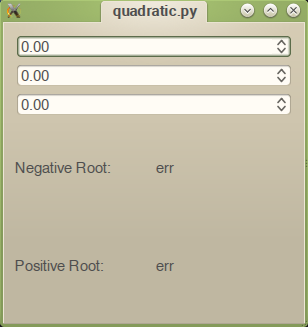
\includegraphics[width=\textwidth]{quadratic_view.png}
\end{subfigure}
\begin{subfigure}[b]{.49\textwidth}
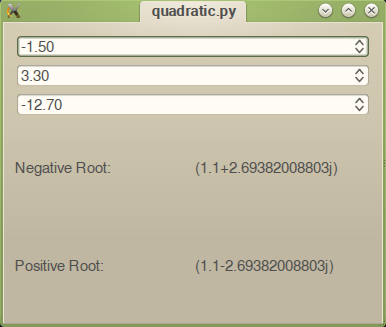
\includegraphics[width=\textwidth]{quadratic_view2.png}
\end{subfigure}
\end{figure}
The widgets that you will need are: \li{QDoubleSpinBox}, \li{QLabel}, \li{QGridLayout}, and \li{QVBoxLayout}.
You can view the documentation for these classes including all methods and signals at \url{http://qt-project.org/doc/qt-4.8/classes.html}
\label{prob:quadCalc}
\end{problem}


\section*{Specifications}

The following is a guideline for your solutions.

\begin{lstlisting}
import sys
from Pyside import QtGui, QtCore

class People(object):
	pass
	
class ComplexNumber(object):
	pass
	
class QuadraticCalculator(QtGui.QWidget):
	pass
\end{lstlisting}

